\begin{question}
Consider the code below.
%
\begin{scala}
var x = 0

def p = proc{ x = x+1; x = x+2 }

def q = proc{ x = x+4 }

def system = p || q
\end{scala}
%
Suppose the atomic actions are reading or writing a variable.
When \SCALA{system} is run, what are the possible final values of \SCALA{x}?
Draw a diagram to illustrate the different possible execution paths.
\end{question}
%
\begin{answer}
The diagram below shows all interleavings until one process terminates, at
which point the system becomes deterministic.  Each label is a triple: the
process doing the event ($P$ or $Q$); an indication of the action (``r'' for
read or ``w'' for write); and the value read or written.  The figures in
circles then show the final value of \SCALA{x} that will result.  The possible
values are 3, 4, 5, 6, 7.  As a check, the diagram shows 
\( {\scriptstyle
  \left( \begin{array}{@{}c@{}} \scriptstyle 6 \\[-1mm] \scriptstyle
    4 \end{array} \right)} = 15 \) interleavings.
%
\begin{center}
\ 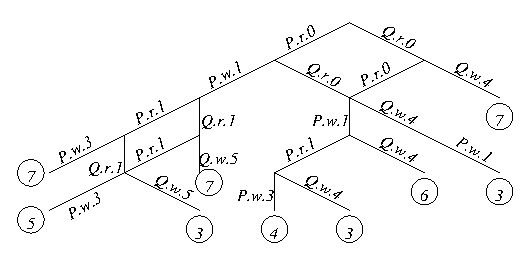
\includegraphics[width=12cm]{interleavings2.eps}\ 
\end{center}
%
The point is that even a very simple program with dependent atomic actions can
become very difficult to understand. 
\end{answer}
